\RequirePackage{luatex85,shellesc}
\documentclass[a4paper,8pt,addpoints,solution]{exam}
\usepackage{pgf,tikz}
\usetikzlibrary{shapes.geometric,automata,arrows,positioning}
\usepackage{tikzsymbols}
\usepackage{marginnote}
\usepackage{pgfplots}
\usepackage{caption}
\usepackage{hyperref}
\usepackage{amsthm}
\usepackage{ulem}
\usepackage{booktabs}
\usepackage{grffile}
\usepackage{amsmath}
\usepackage{mathtools}
\usepackage{amssymb}
\usepackage{tcolorbox}
\usepackage{fontspec}
% \setmainfont{opensans}
% \usepackage[euler-digits]{eulervm}
% \usepackage{libertine}
\usepackage{pgfplots}
\usepackage{epsdice}
\usepackage{tfrupee}
\usepackage[top=2cm, bottom=2cm, left=3cm, right=5cm, heightrounded,
      marginparwidth=4cm, marginparsep=5mm]{geometry}

\newcommand\MEAN[1]{\langle #1\rangle}
\newcommand\VAR[1]{\text{Var}(#1)}
\newcommand\BONUS{\textbf{(bonus)} }
\newcommand\MARGIN[1]{\marginpar{\emph{\small #1}}}
\newcommand\PR{\text{Pr}}

% solution.
\printanswers

% Title Page
\title{Information Theory 2019 \\ Tutorial 1} 
\author{Dilawar Singh}
\date{\today}
\begin{document}
\maketitle

\section{Probability}

\begin{itemize}
    \item $\Omega$ : Set of all possible outcome.
    \item $Pr(x)$, probability of event $x$. $x$ must be in $\Omega$ (i.e., $x \in \Omega$).
    \item  Sum of $Pr(x)$ for all $x$ in $\Omega$ must add to to 1 or,
        mathematically, $\sum_{x\in\Omega} Pr(x)= 1$ \footnote{You will see
        $\sum$ more often in the course. Familiarize yourself with $\sum$}
\end{itemize}

For example, when I roll a die it can land in six ways. For such a  die,
$\Omega$ consists of six outcomes (elements).  $\Omega={ \epsdice{1},
\epsdice{2}, \epsdice{3},\epsdice{4},\epsdice{5},\epsdice{6} }$. When die is
fair, all outcomes are equally likely i.e. $Pr(\epsdice{1}) = Pr(\epsdice{2}) =
\ldots = Pr(\epsdice{6})$. Also $Pr(\epsdice{1}) + Pr(\epsdice{2}) + \ldots +
Pr(\epsdice{6}) = 1$. These two facts implies that any outcome has the
probability of $\frac{1}{6}$ or $Pr(x) = \frac{1}{6}$,  $\forall x\in\Omega$
($\forall$ is shorthand for `for all').

\paragraph{Mean and Variance} There are three prominent ways to compute/estimate
the 'average': mean, mode and median. We'll focus on mean here since it turns
out to be the more meaningful in applications than the rest. Mean is also called
expected value \MARGIN{I get it: On average, ``average'' means ``mean''}.  For a random
variable $X$, we shall use the symbol $\MEAN{X}$ to denote the mean (expected
value) of it. The variance of $X$ (often denoted by $\VAR{X}$) is the measure of
variability in the random variable $X$. It is defined as the mean square
deviation from the mean. $\VAR{X} = \MEAN{X - \MEAN{X}}^2$ (see problem 2).

Two random variables $X$ and $Y$ are called independent if the output of one
does not depend on the outcome of other. 

\subsection*{Problems}
\begin{questions}

    \question Mean and variance
    \begin{parts}
        \part[1] What is the expected value of a pair of dice.
        \begin{solution}
            The expected value of sum of two random variables is equal 
            to the sum of expected value of each one ie., $\MEAN{X_1+X_2}=\MEAN{X_1}+\MEAN{X_2}$.
            Below is a simulation of two dice rolled for over 10000 times. The
            expected value of both dice is plotted. It converges to 7.

            \begin{tikzpicture}[]
                \begin{axis}[xlabel=N, ylabel=Expected Value, grid]
                    \addplot [color=blue, very thick
                        , error bars/.cd, y dir=both, y explicit
                        ]
                        shell [prefix=prob1] {python mean_dice.py};
                \end{axis}
            \end{tikzpicture}	
        \end{solution}
        \part[5] Why do we care about variance? Everyone computes it but what is
        so natural about it? (Hint:
        $Pr\left((X-\MEAN{X})^2 \ge \alpha \right) \le \VAR{X}/\alpha$ [Chebyshev 1963]) 

        \begin{solution}
            Variance of a random variable has this very useful property
            $Pr\left((X-\MEAN{X})^2 \ge \alpha \right) \le \VAR{X}/\alpha$,
            for all $\alpha$; which very roughly says that a random variable
            $X$ will rarely be far from its mean $\MEAN{X}$ if its variance
            $\VAR{x}$ is small.

            Technically, if you care for a proof.
            \begin{proof}
                Convince yourself that following two definitions of variance
                are the same.
                \begin{enumerate}
                    \item $\VAR{X}=\sigma^2=\MEAN{(X-\MEAN{X})^2}$
                    \item $\VAR{X}=\sigma^2=\sum\limits_{\omega \in \Omega} (X(\omega)-\MEAN{X})^2
                        Pr(\omega)$. Or in the notation of class
                        $\VAR{X}=\sum\limits_{p_i} (x_i - \mu)^2p_i$ where $\mu$
                        is $\MEAN{X}$ and $p_i$ is the probability of occurrence
                        of symbol $x_i$. We are going to use this definition.
                \end{enumerate}

                \begin{align}
                    \VAR{X} = \sigma^2 
                        &= \sum\limits_{p_i} (x_i - \mu)^2 p_i \\
                        & \ge \sum\limits_{\substack{p_i \\ (x_i-\mu)^2 \ge \alpha}} (x_i - \mu)^2 p_i \\
                        & \ge \sum\limits_{\substack{p_i \\ (x_i-\mu)^2 \ge
                            \alpha}} \alpha p_i = \alpha \PR\left((X-\mu)^2 \ge
                        \alpha\right) \label{eq1}
                \end{align}

                Let's use $\alpha=c^2\sigma^2$, we get $(X-\mu)^2 \ge
                c^2\sigma^2$. Equation \ref{eq1} turns into 
                $\PR(|X-\mu|\ge c\sigma) \le 1/c^2$. 

                Thus, the probability that $X$ will lie within $c$ standard deviations of its mean
                is at least $1-1/c^2$. A random variable will lie within
                2$\sigma$ of $\mu$  at least 75\% ($1-1/4$) of time. This is
                true of all distribution. Recall for normal distribution, this
                value is 95\%. Wikipedia article on Chebyshev inequality has
                more discussion about it.
            \end{proof}
        \end{solution}

    \end{parts}


\question[5] Prove of disprove: If $X$ and $Y$ are independent random variables,
then so are $F(X)$ and $G(Y)$ where $F$ and $G$ are any function. 

\begin{solution}
    This sound obvious and it is true but the proof can be bit confusing. 
    \begin{proof}
        You can write it in your own words as well. For obvious reason, $F$ and $G$ must
        be defined over all possible $x_i$ and $y_i$.
        \begin{align}
            \PR\left(F(X)=f\;\text{and}\; G(Y)=g\right) 
                &= \sum\limits_{\substack{x\in F^{-1}(f) \\ y\in G^{-1}(g)}} \PR(X=x\;\text{and}\;Y=y) \\
                &= \sum\limits_{\substack{x\in F^{-1}(f) \\ y\in G^{-1}(g)}}
                    \PR(X=x)\cdot\PR(Y=y) \\
                &= \PR(F(X)=f) \cdot\PR(F(G)=g)
        \end{align}
    \end{proof}
\end{solution}

\bonusquestion[3] Construct a random variable which has finite mean and infinite
variance.
\begin{solution}
    Not given.
\end{solution}

\question[10]
Two lotteries sells 100 tickets every week. At the end of the week, one of these
tickets is selected randomly (each ticket is equally likely to win) and winner
is given 1 lakh rupees. Other 99 tickes gets nothing. You have enough money to
buy two tickets: you can buy both tickets from the same lottery or 1 from each
lotteries. Which strategy is \textit{better} given that you can play lottery enough
time.

\begin{solution} 
    If we buy two tickets from the same lottery (strategy \textbf{S1}), we have
    2\% chance of winning \rupee 1 lakh, and 98\% change of winning nothing.  If
    we buy both tickets from different lotteries (strategy \textbf{S2}), we have
    some change of winning \rupee 2 lakhs. Lets write down the probabilities.

    \begin{tabular}{c c c c}
        Strategy                    & \rupee 0     & \rupee 1 lakh & \rupee 2 lakh \\
        S1                          & 0.98         & 0.02          & \\
        S2                          & 0.9801       & 0.0198        & 0.0001 \\
    \end{tabular}

    With S2, we have slightly higher chance of not winning anything. But a non-zero
    chance of winning \rupee 2 lakhs. The expected value of win (mean) is same is
    both cases: $0 \times 0.98 + 0.02 \times 1 = 0.02$, and $0\times 0.9801 + 0.0198
    * 1 + 0.0001 * 2 = 0.02$. Yet the strategy looks different. After all if I buy
    100 tickets from same lottery, I am sure to win \rupee 1 lakh, but not with S2.

    Strictly speaker, which strategy is better is beyound the scope of this
    tutorial. All we can show how to do the calculations.  The standard deviation of
    S1 is ($\sqrt{0.98(0-0.02)^2+0.02(1-0.02)^2}$) 0.1386 and of S2 is
    0.1392265. We can say that S2 is \rupee 0.0006265 lakh riskier.

    Let play this lottery on computer since we can not play in real life.
    Figure \ref{fig:lottery} shows the simultion. More often than not, S2 gives
    slightly higher return.

    \includegraphics[width=1\textwidth]{./lotteries.py.png}\label{fig:lottery}
    \captionof{figure}{Second strategy is slightly better. On average, we might win more
        money with S2 given that we win \rupee 2 lakh. For very large number (almost
        infinite), both strategy will yield same results (since mean is same), however
        for large numbers of times lottery played, S2 seems to be more beneficial (as
    per simulations).}

\end{solution}

\question For a pair of dice, write $\Omega$.
\begin{parts}
    \part[2] Consider $\epsdice{1}\epsdice{4}$ and $\epsdice{4}\epsdice{1}$ etc. as distinct events.
    \part[3] Consider $\epsdice{1}\epsdice{5}$ and $\epsdice{5}\epsdice{1}$ etc. as same event.
    \part[3] \textbf{(bonus)} Repeat the problem for 4 dice. You can use computer program to
check your results.
\end{parts}

\question[5]
Your TA flipped a Rs. 1 coin repeatedly. Once he got two head in succession,
he noted down the number of flips. He got the following sequence:
\verb|6,3,6,8,7,12,16,2,3,2| 
Fortunately others have also done such exercise. I was able to get following
data from two universities.

\begin{itemize}
    \item \verb|3,2,3,5,10,2,6,6,9,2|     (Stanford, 1979)
    \item \verb|10,2,10,7,5,2,10,6,10,2|  (Princeton, 1987)
\end{itemize}

\begin{parts}
    \part[2] Compute (umm. estimate) the mean and variance of these sequences.
    \bonuspart[3] Based on these sequence, can you estimate the
    probability that coin used was not 'fair'? If yes, estimate. If no, why not?
\end{parts}

\begin{solution}
\begin{tabular}{c c  c}
 Coin         & mean & $\sqrt{\text{variance}}$ \\
NCBS 2017     & 6.5  & 4.34  \\
Stanford 1979 & 4.79 & 2.78  \\
Princeton 1987& 6.4  & 3.35  \\
\end{tabular}

The answer is no and its not easy to explain.
Lets call this process X. Lets take an extreme case: NCBS 2017 series was the
following: 2,2,2,2,2,2,2,2,2,2 i.e. all 20 flips gave us heads. Can we say this
was definately a loaded coin? What is the probability that this sequence came
out of a fair coin? Or what is the probability of getting 20 heads in
succession? Ans is $(\frac{1}{2})^{20}$. It is non-zero!

What is the mean and variance of X for a fair coin anyway?  \footnote{mean=6,std=4.7}
\end{solution} 

\question[10] \textbf{Ultimate Frisbee} 
\sout{Six} Five players stand at the vertices of a \sout{hexagon} pentagon, throwing
Frisbees to each other.

\tikz{
    \node[draw, regular polygon, blue, regular polygon sides=5, inner sep=1cm] (a) {};

    \tikzset{frisbee/.style={-latex, very thick, shorten <= 2pt}}
    \node[circle, fill=blue] (p1) at (a.corner 1) {};
    \node[circle, fill=blue] (p2) at (a.corner 2) {};

    \draw[frisbee] ([shift=(45:1mm)]p1) -- ++(-60:7mm);
    \draw[frisbee] ([shift=(45:1mm)]p1) -- ++(210:7mm);

    \draw[frisbee] ([shift=(45:1mm)]p2) -- ++(45:7mm);
    \draw[frisbee] ([shift=(45:1mm)]p2) -- ++(-60:7mm);
}

They have two Frisbees, initially at the adjacent vertices as shown in the
figure above. The Frisbee is thrown either to the left or to the right with
equal probability. The game stops when one player is the target of both
Frisbees. (All throws the independent of past history).

\begin{enumerate}
    \item Find the mean and variance of the number of pairs of throws. For some
        initial values, the game may never stop in the case of hexagon.
    \item Find the expression for probability that the game lasts more than 500
        steps, in terms of Fibonacci numbers.
\end{enumerate} [Conc. Math., Knuth]

\begin{solution}
    \emph{In the original draft of this tutorial, I used a hexagon. For the
        given initial condition, the game will never stop. Or it will always
        take more than 500 steps.
    }

    The solution to this problem is tricky. I could not find a solution
    different than one given in the reference which use probability generating
    function.\footnote{What is the probability of getting such a complicated problem in
    your tutorial?}

    There are various ways to setup this problem. Here is mine. Lets define the
    states of the system. One can use vertices of the pentagon. A more useful
    one would be the distance between frisbees. There are tree states: distance
    of 0, 1, and 2. The state transition diagram is following where number on
    the arrows are the probability of transition.

    \tikzset{state/.style={circle,fill=blue!20, draw=none}}
    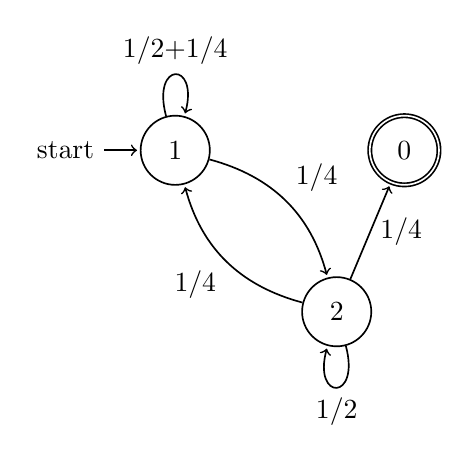
\begin{tikzpicture}[semithick, node distance=2cm, auto, shorten >= 1pt]
        \node[initial,state] (n1) {1};
        \node[state,right=of n1, accepting] (n0) {0};
        \node[state,below right=of n1] (n2) {2};

        \path[->] 
            (n1) edge[bend left] node {1/4} (n2)
                edge[loop above] node {1/2+1/4} ()
                (n2) edge[bend left] node {1/4} (n1)
                edge[loop below] node {1/2} ()
                edge node[right]{1/4} (n0);
    \end{tikzpicture}	

    If we walk on this state machine (always from \tikz \node[state] {1};), we
    get sequence of nodes. For example, 120, 1220, 12220, 12120 etc. By looking
    at this picture, we can say few things. First, possibility of a game lasting
    N steps is non-zero for all N (we can get stuck in state \tikz \node[state]
    {2}; or \tikz\node[state]{1}; for as long as we like with non-zero
    probability).

    \paragraph{Mean and variance of pairs of throw} Its rather simple but
    counting is hard! Enumerate all paths which starts from
    \tikz\node[state]{1}; and end with \tikz\node[state]{0}; and note down their
    probability and length. For example, path \texttt{120} has length 2 and probability
    of 1/16; similarly path \texttt{12120} has length 5 and probability
    1/4$\cdot$1/4$\cdot$1/4$\cdot$1/4=1/256. Other examples are 120, 1120,
    11120, 11220, 11220, etc.. Unfortunately there is no simple argument by
    which we can ignore some paths.

    I used computer to simulate the game as it is; and also to simulate the state
    machine shown above. I got roughly the same answer.

    \begin{tabular}{l l l}
         & Mean & std \\
        State Machine & 12.9657 & 10.0026 \\
        Game & 12.970 & 9.936965
    \end{tabular}

    The Python3 script can be found here
    \url{http://github.com/dilawar/courses/raw/master/TASHIP/InformationTheory2019/Tutorial1/frisbee.py}.

    \paragraph{Generating function} You will meet the probability generating
    function later in the course but don't worry; we don't ask any question
    about them in the exam. But they are powerful abstraction. And this
    exercise should convince them. For the above state machine, lets say there
    are three generating function A (distance 0), B (distance 1), and C
    (distance 2) where $z^nB$ would mean the probability of distance 1 after n
    throws. The generating function satisfies the following (look at the state
    machine).

    $$A = \frac{1}{4}zB$$ meaning Pr(\tikz\node[state]{2}; $\rightarrow$
    \tikz\node[state]{0};)=1/4. Or if both frisbees are already 1 distance away,
    and probability of zero distance between them after one throw is 1/4,
    similarly, 

    $$B=\frac{1}{2}zB + \frac{1}{4}zC,\quad C=1+\frac{1}{4}zB+\frac{3}{4}zC$$
    
    And we are done. It follows that $A=\frac{z^2}{16-20z+5z^2}$. Computing mean
    and variance of A is straightforward once you know the basic theory behind
    z-transform. The results are mean=12 and variance=100.

    If you have a simpler solution, that would be really cool!

\end{solution}

\paragraph{Typical dressing}

\question[5] \textbf{(Counting)}
A man has a non-magical wardrobe containing 10 shirts, 10 pants, 20 pairs of
socks, 10 pairs of shoes, 30 hats, and 50 neck-ties. He picks 6 items everyday.
Whenever he picks 1 shirt, 1 pant, 1 pair of shoes, 1 pair of socks, 1 hat and
1 neck-tie, we call is 'typical dressing'.

\begin{parts}
    \part[2] How many ways he can choose 6 items? 
    \begin{solution}
        There are total 130 items.  For first item, we have 130 choices,
        for second item, we have 129 choices etc. Total choices are $130 \times 129
        \times 128 \ldots 125$.
    \end{solution}

    \part[3]How many ways he can dress himself 'typically'?
    \begin{solution}
        He has to pick 1 items of each type. How many ways he can choose 1
        shirt out of 10 shirts? 10. Similarly there are 30 ways to pick 30 hats etc.
        Total typical dressings are $10 \times 10 \times 20 \times 10 \times 30 \times
        50$.
    \end{solution}

    \part[3] In a slightly off-beat world, a typical dressing contains at least 1
    shirt, 1 pant, and 1 pair of shoes. Rest of the 6 garments could be
    anything else. How many ways he can dress himself 'typically'?
    \begin{solution}
        Let assume that he picks required 1 shirt first. There are 10 ways. Next he
        picks required 1 pant, there are 10 ways. Similarly there are 10 ways for
        picking required 1 pair of shoes. Left are 3 garments and they could be anything.
        How many ways he can pick 3 items out of 9 shirts, 9 pants, 10 pairs of shoes,
        20 pairs of socks, 30 hats and 50 neck-ties (total 127). Go back to problem 1. Ans is 
        $127 \times 126 \times 125$ for this part. So total ways to dress oneself
        typically is $10 \times 10 \times 10 \times 127 \times 126 \times 125$.
    \end{solution}
\end{parts}

\section{Distributions} \question[5] A man claims that he has average height and
average weight, therefore, he is an average man. But he is considered slightly
overweight. Explain? (Hint: Weight $\propto$ height$^3$)

\begin{solution}
    Jensen Inequality which state that if $f$ is a convex function then
    $f(\MEAN{X}) \le \MEAN{f(X)}$. It follows $\MEAN{X}^3 \le \MEAN{X^3}$
    i.e., weight for the average height is less than the average weight of the
    population. 
\end{solution}

\section{Some calculus}

\question $log_2 x = n \iff 2^n = x$
\begin{parts}
    \part[1] Show/prove/argue that $0 \log 0 = 0$.
    \part[2] Show that $\log_x y = \frac{\log_a y}{\log_a x}$.
    \part[2] Plot (show your work) $x \log(x) + (1-x) \log (1-x)$ where $0 \le x \le 1$.
\end{parts}

\begin{solution}
Solution Not given.
\end{solution}

\end{questions}

\end{document}          
